\ifnum \Version=7
\question[2] Suppose $\displaystyle \dydt =y^2(y-4)$. Determine all possible values $y$, if any, where solution curves will tend to $y=0$. Please show your work. 

\ifnum \Solutions=1 {\color{DarkGreen} 
\textbf{Solutions:} \\
If we sketch the phase line we obtain:

\begin{center}
    \begin{tikzpicture}[ultra thick]
    \DrawHorizontalPhaseLine[$y$]{0,4}{5}{-1,2}%
\end{tikzpicture}
\end{center}

The critical points are:
\begin{itemize}
    \item $y=0$ which is semi-stable
    \item $y=4$ which is unstable
\end{itemize}
The values of $y$ where the solutions tend to $y=0$ are on the interval $[0,4)$. We can't include $y=4$. We can also express the answer as
$$0\le y < 4$$
} 
\else 
\vspace{6cm}
\fi\fi 



\ifnum \Version=9
\question[2] Suppose $\displaystyle \dydt = y(4-y)^2$. Determine all possible values $y$, if any, where solution curves will tend to $y=4$. Please show your work. 

\ifnum \Solutions=1 {\color{DarkGreen} 
\textbf{Solutions:} \\
If we sketch the phase line we obtain:

\begin{center}
    \begin{tikzpicture}[ultra thick]
    \DrawHorizontalPhaseLine[$y$]{0,4}{2,5}{-1}%
\end{tikzpicture}
\end{center}

The critical points are:
\begin{itemize}
    \item $y=0$ which is unstable
    \item $y=4$ which is semi-stable
\end{itemize}
The values of $y$ where the solutions tend to $y=4$ are on the interval $(0,4]$. We should include $y=4$, and we can't include $y=0$. We can also express the answer as
$$0 < y \le 4$$
} 
\else 
\vspace{6cm}
\fi\fi 



\ifnum \Version=8
\question[2] Suppose $\displaystyle \dydt = y(1-y)(2-y)$. Determine all possible values $y$, if any, where solution curves will tend to $y=1$. Please show your work. 

\ifnum \Solutions=1 {\color{DarkGreen} 
\textbf{Solutions:} \\
If we sketch the phase line we obtain:

\begin{center}
    \begin{tikzpicture}[ultra thick]
    \DrawHorizontalPhaseLine[$y$]{0,1,2}{0.5,2.5}{-1,1.5}%
\end{tikzpicture}
\end{center}

The critical points are:
\begin{itemize}
    \item $y=0,2$ which are unstable
    \item $y=1$ which is stable
\end{itemize}
The values of $y$ where the solutions tend to $y=1$ are on the interval $(0,2)$. We should not include $y=0$, and we can't include $y=2$. We can also express the answer as
$$0 < y < 2$$
} 
\else 
\vspace{6cm}
\fi\fi 

\ifnum \Version=6
\question[2] Suppose $\displaystyle \dydt = y(y-4)(y-6)$. Determine all possible values $y$, if any, where solution curves will tend to $y=4$. Please show your work. 

\ifnum \Solutions=1 {\color{DarkGreen} 
\textbf{Solutions:} \\
If we sketch the phase line we obtain:

\begin{center}
    \begin{tikzpicture}[ultra thick]
    \DrawHorizontalPhaseLine[$y$]{0,4,6}{2,7}{-1,5}%
\end{tikzpicture}
\end{center}

The critical points are:
\begin{itemize}
    \item $y=0,6$ which are unstable
    \item $y=4$ which is stable
\end{itemize}
The values of $y$ where the solutions tend to $y=4$ are on the interval $(0,6)$. We should not include $y=0$, and we can't include $y=6$. We can also express the answer as
$$0 < y < 6$$
} 
\else 
\vspace{6cm}
\fi\fi 

